\section{Methods of signal reconstruction}
\label{sec:signal}

Unlike the resistance of bolometers that can be directly measured to return a signal proportional to the incident power, the monitoring of the resonance of a KID requires a more complex readout scheme. In fact, one of the challenges of operating a KID is to convert the \I$(t)$ and \Q$(t)$ values to an absorbed optical power or shift in resonant frequency as a function of time $\delta f_{0} \propto \delta P_{opt}$. In this
section, we will see how to adress this problem by using a new modulated readout technique and then by using two different signal reconstruction methods : \rf\ and \cf.

\subsection{Modulated readout technique}
An innovative readout technique has been developed to monitor the change of the signal by using a known frequency shift. The standard excitation of the detectors with a fixed tone is replaced by a new excitation based on two different frequencies. The local oscillator is modulated between two values, separated by $\delta f_{LO} \simeq 1$ kHz, and provides $f_{+} = f_{0} + \frac{\delta f_{LO}}{2}$ and $f_{-} = f_{0} - \frac{\delta f_{LO}}{2}$ with $f_{0}$ the detector resonant frequency.\\
The values ($I(t)$,$Q(t)$) are then given by :

\begin{equation}
(I(t),Q(t)) = (\frac{I(f_{+}) + I(f_{-})}{2}, \frac{Q(f_{+}) + Q(f_{-})}{2}),
\end{equation}

and the differential values are :

\begin{equation}
\label{gradient}
(\delta I(t), \delta Q(t)) = (\frac{I(f_{+}) - I(f_{-})}{\delta f_{LO}}, \frac{Q(f_{+}) - Q(f_{-})}{\delta f_{LO}}).
\end{equation}

\begin{figure}[h]
\center
	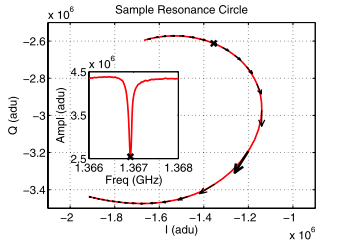
\includegraphics[scale=0.8]{Figures/resonance-circle.png}
	\caption{Representation in the \I\ - \Q\ plane of a frequency sweep around a resonance. The red line represents the $(I,Q)$ data of the frequency sweep around the resonance. The arrows represent (\di, \dq). \citep{2013A&A...551L..12C}}
	\label{circle-iq}
\end{figure}

Fig. \ref{circle-iq} shows a typical KID resonance circle. Thanks to this
modulation technique, we obtain four quantities : \I\ , \Q\ and their variation
$\delta I$, $\delta Q$.\\ In this paper, \I$(t)$ and \Q$(t)$ are sampled at 22 Hz,
they are the mean values of sub-sample $i(t)$ and $q(t)$ on $N_{m}$ = 40 points at
880 Hz. \di$(t)$ and \dq$(t)$ are the mean values of the difference between the data
measured at $f_{-}$ and $f_{+}$ :

\begin{eqnarray}
I  &=& \sum^{N_{m}=40}_{p=1} i_{p},\\
%\label{eq:i}
Q  &=& \sum^{N_{m}=40}_{p=1} q_{p},\\
%\label{eq:q}
dI &=& \sum^{N_{m}/2=20}_{p=1} i_{2p} - i_{2p-1},\\
dQ &=& \sum^{N_{m}/2=20}_{p=1} q_{2p} - q_{2p-1},
\end{eqnarray}

% on voit les equations \ref{eq:i}, \ref{eq:q}.\\

With these quantities in hand we have several ways to derive the transmitted signal. They are presented in the following paragraph.

\subsection{RfdIdQ}
If a variation \di$(t)$, \dq$(t)$ is observed between successive  ($I(t)$, $Q(t)$) points, it is possible to estimate the shift of the resonant frequency $\delta f_{0}$ between two samples by comparing ($\Delta I(t)$, $\Delta Q(t)$) with the gradient $(\delta I(t), \delta Q(t)) $ induced by the known $\delta f_{0}$ of the local oscillator. This is done by projecting ($\Delta I(t)$, $\Delta Q(t)$) along the gradient found in Eq.~(\ref{gradient}). $\delta f_{0}$ is then determined by integrating Eq.~(\ref{eq:Rf}) \citep{2014A&A...569A...9C}.

\begin{equation}
\label{eq:Rf}
\Delta f_{0} = \delta f_{LO} \frac{\Delta I < I >_{50} + \Delta Q < Q >_{50}}{< I >_{50}^{2} + < Q >_{50}^{2}},
\end{equation}

%\delta f_{LO} \frac{\Delta I <dI>_{50} + \Delta Q <dQ>_{50}}{<dI>_{50}^{2} + <dQ>_{50}^{2}}

where $<.>_{50}$ means that we average the considered quantities over 50 points before and after the concerned value, and $\delta f_{LO} \simeq 1$ kHz.

This method is convenient, but can be affected by some systematic uncertainty and be a source of non-linearity. In fact, $(\delta I(t), \delta Q(t))$ is tangent to the (\I,\Q) circle for a fixed background optical power, whereas the actual variation ($\Delta I$, $\Delta Q$) occurs for a fixed excitation frequency and is due to a difference in the optical power, that includes a change in the (\I,\Q) circle radius. As a consequence, the observed (\I,\Q) trajectory is not precisely parallel to the direction given by $(\delta I(t), \delta Q(t))$. The predicted error induced by the projection method is less than 2\% for faint sources \citep{2013A&A...551L..12C}.

\subsection{Circle fit : Cf}
To improve \rf, we developed a new technique named \cf.\\
The idea of this method is to project \I,\Q, \di, \dq, onto an axis named $y'$ which is as linear as possible with frequency, and so is assumed to be linear with the optical power. To do so we study the quantity $Z=I+jQ$, which near a resonance is on a circle. We suppose that :

\begin{equation}
f - f_{0}= \frac{w}{2} \tan \frac{\phi}{2}.
\label{eq:hyp-f}
\end{equation}

The idea is to construct $y'$ from a circle $Z$. The inverse of $Z$ is a circle but we can normalize it to transform it into an infinite radius circle that is expected to be linear with the KID frequency.  To do so we define a reference circle which is centered on ($\frac{1}{2},0$) and has a radius of $\frac{1}{2}$, after using trigonometric relations we obtain : 

\begin{equation}
Z_{ref} = \cos \frac{\phi}{2} exp j \frac{\phi}{2}.
\label{eq:Zref}
\end{equation}

If we inverse Eq.~(\ref{eq:Zref}), we have : 
\begin{equation}
Z_{res} = 1 - j \tan \frac{\phi}{2}.
\label{eq:Zres}
\end{equation}

The imaginary part of Eq.~(\ref{eq:Zres}) is linearly dependant on the frequency defined in Eq.~(\ref{eq:hyp-f}), and represents the new axis $y'$.

From the KID model we have $Z=I+jQ$. We do a series of transformations on this circle to make it identical to the reference circle, the final result is named $Z'$, with $Z'=p[ZM_{r} + T]$. p is the scaling factor, T represents the translation and $M_{r}$ is the rotation matrix : 

\begin{equation}
M_{r} = 
\begin{pmatrix}
	\cos \alpha & \sin \alpha \\
	-\sin \alpha & \cos \alpha
\end{pmatrix} .
\end{equation}


First we rotate $Z$ :
\begin{equation}
Z' = 
\begin{pmatrix}
	\cos \alpha & \sin \alpha \\
	-\sin \alpha & \cos \alpha
\end{pmatrix}
\begin{pmatrix}
	I\\
	Q
\end{pmatrix}
=
\begin{pmatrix}
	I\cos \alpha + Q\sin \alpha\\
  - I\sin \alpha + Q\cos \alpha
\end{pmatrix}.
\end{equation}

Then we translate and rescale it, to obtain $Z'=I'+jQ'$ with : 
\begin{eqnarray}
I' &=& \frac{1}{2r}[(I-x_{c}) \cos \alpha + (Q - y_{c}) \sin \alpha] + \frac{1}{2}, \\
Q' &=& \frac{1}{2r}[-(I-x_{c}) \sin \alpha + (Q - y_{c}) \cos \alpha]. \\
\end{eqnarray}

($x_{c}, y_{c}$), r and $\alpha$ respectively, the center, radius and rotation angle of the initial circle. The derivative of the inverse of $Z'$ is $dZ_{res}=-dZ'/Z'^{2}$, with :

\begin{eqnarray}
dZ' &=& dI' + jdQ',\\
dI' &=& -\frac{1}{2r}(dI \cos \alpha + dQ \sin \alpha), \\
dQ' &=& \frac{1}{2r}(-dI \sin \alpha + dQ \cos \alpha).
\end{eqnarray}

The imaginary part of $Z_{res}$ and $dZ_{res}$ represent respectively $y'$ and $dy'$ which are proportional to the KID frequency. We can use these quantities to calibrate $y'$ and derive the frequency of the KID. In fact, according to the hypothesis in Eq.~(\ref{eq:hyp-f}), $f$ is a polynomial, so to reconstruct the shift of the resonant frequency we can fit $\frac{\Delta f}{dy_{3}} = R_{n}(y')$ by a polynomial function, where $R_{n}$ is a polynomial function with a degree $n$. It is then easy to integrate $R_{n}$ into $P_{n+1}$, with $\overset{.}{P_{n+1}}=R_{n}$  to obtain the relative frequency of the KID : 

\begin{equation}
f - f_{0} = P_{n+1}(y')
\end{equation}

In conclusion, because we can not directly measure the optical power from a KID, new methods were developped to monitor the shift of the resononance frequency of the detector. First with the modulated readout technique we can calculate four quantities : \I, \Q, \di, \dq. With these quantities in hand, we can monitor the shift of the resonant frequency and derive the corresponding incident power ny using the two methods that were developped : \rf\ which is already successfully used in \nika\ and \nika2\ (see \citep{2014A&A...569A...9C}) , and \cf\ which is an improvement from \rf . In this paper, we compare these two methods in terms of linearity. To do so, in the next sections we do simulations of observations by a KID and we use \rf\ and \cf\ to reconstruct the signal. We then study the impact of the KID non-linearity on the search for B modes polarization of the CMB.